\documentclass[10pt]{article}
\usepackage[english]{babel}
\usepackage[utf8x]{inputenc}
\usepackage{amsmath}
\usepackage{graphicx}
\usepackage{caption}
\usepackage[colorinlistoftodos]{todonotes}
\usepackage{indentfirst}
\usepackage{geometry}
\usepackage[section]{placeins}
\usepackage{float}
\geometry{letterpaper, portrait, margin=1in}
\usepackage{hyperref}
\usepackage{subfigure}
\title{Autonomous- Final Report}
\addcontentsline{toc}{section}{References}
\begin{document}

\begin{titlepage}

\newcommand{\HRule}{\rule{\linewidth}{0.5mm}} % Defines a new command for the horizontal lines, change thickness here
\center % Center everything on the page
\textsc{\Large ECE 592-063 Introduction to Autonomous Systems}\\[1.5cm]
\HRule \\[0.4cm]
{ \huge \bfseries Final Report 

Indoor SLAM -2 using Visual SLAM}\\[0.4cm] % Title of your document
\HRule \\[1.5cm]
\begin{minipage}{0.4\textwidth}
\begin{flushleft} \large
\emph{Authors:}\\
Suraj Shanbhag % Your name

Abhishek Ravi	 % Your name

William Burdick-Crow % Your name

Siddharth Ganesh % Your name

\end{flushleft}
\end{minipage}
~
\begin{minipage}{0.4\textwidth}
\begin{flushright} \large
\emph{Mentor:} \\
Dr.Mihail L. Sichitiu % Supervisor's Name
\end{flushright}
\end{minipage}\\[0.5cm]
{\large April 23,2017}\\[2cm] 

\includegraphics[width=10.5cm]{n.png} % Include a department/university logo - this will require the graphicx package
 
%----------------------------------------------------------------------------------------
\vfill % Fill the rest of the page with whitespace

\end{titlepage}

\tableofcontents



\listoffigures



\listoftables
\pagebreak
\section{Abstract}
	Incorporating computer vision on any system requires an immense computation power, which increases the cost and size of the system. For small robots and airborne drones it might not always be feasible to add more computation power. In this report we suggest a system where the processing of the stereo camera video feed is offloaded to a remote computer running ROS whose performance can be scaled to match the task. We use a small 2 wheeled robot with the 2 cameras and a Raspberry Pi 3 to stream the stereo video feed to the host computer which performs the tasks. Other challenges like synchronization, calibration and quality of the video are also addressed in the report. The stereo video feed received is used to create a map of the environment and help the robot navigate. This system becomes a good platform to test various Visual SLAM algorithms and we have tested ORBSLAM2 and RTAB.



\section{Introduction}
Although existing technology has made great leaps and bounds in mapping outdoor areas, it still hasn't made much progress in mapping an indoor environment. This is mainly because of the large size of the current robots being used for mapping making them un-traversable in constrained and small spaces. When such a problem arises, it is convenient if we figure out a way to map our entire surroundings so that we can have a reference to work with and make informed decisions. This problem of indoor or constrained SLAM is of extreme importance in disaster management and medical applications. By gaining real world data of these areas we can actually get an insight into the environment, be it a building debris or the inside of the intestines. By implementing visual SLAM on a two wheeled mobile robot we are presenting a case that, the robot need not be as powerful in itself to perform such high computational problems but can act as a carrier of message to a powerful system to solve real world problems.

	Currently there is very little support for using ROS to run remote slam operations. A large part of our project has been, enabling the usage of remote processing on these ROS applications. This allows for increased flexibility, both in type and cost, of the type of vehicle used for capturing images. It will also allows for a much cheaper vehicle, as all that the vehicle is responsible for is streaming the images back to the computer and controlling the robot. Due to the very few requirements that we have for the robot, it is easy to change what platform is used to carry the camera. As long as the robot is capable of streaming video, our project is applicable.


\section{Related work}
Although nobody has published their findings of Visual Stereo SLAM on a Raspberry pi, we found a work on monocular SLAM using Raspberry pi camera module.\footnote{\href{https://courses.cit.cornell.edu/ece6930/ECE6930\_Spring16\_Final\_MEng\_Reports/SLAM/Real-time\%20ROSberryPi\%20SLAM\%20Robot.pdf}{https://courses.cit.cornell.edu/ece6930/ECE6930\_Spring16\_Final\_MEng\_Reports/SLAM/Real-time\%20ROSberryPi\%20SLAM\%20Robot.pdf}}
This work basically revolves around using a raspberry pi+ camera module on a two wheeled robot of raspberry pi for loop detections and re-localization using ORBSLAM while streaming at a much low image quality for a single camera to find loop closure and odometry. Monocular SLAM can be handled by a raspberry pi, but streaming two video streams for stereo ORBSLAM is complex. There is extensive research and findings publicly available for pre-built stereo cameras but none for an assembled stereo camera setup using two monocular USB cameras. People have eliminated the use of two USB Cameras connected to a pi by using the Pi compute module. This eliminated the time synchronization issues and gives a very good image resolution.\footnote{\href{http://hackaday.com/2014/11/03/stereo-vision-and-depth-mapping-with-two-raspi-camera-modules/} {http://hackaday.com/2014/11/03/stereo-vision-and-depth-mapping-with-two-raspi-camera-modules/}} An already implemented SLAM algorithm for Stereo Outdoor mapping  \footnote{\href{http://wiki.ros.org/rtabmap\_ros}{http://wiki.ros.org/rtabmap\_ros}} served as a guide for our project to implement a low cost Indoor stereo SLAM. RTABMap (Real Time Appearance Based Mapping) is used widely to reconstruct our 3D environment. It has been deployed using a bumblebee stereo camera.\footnote{\href{http://wiki.ros.org/rtabmap\_ros/Tutorials/StereoOutdoorMapping}{http://wiki.ros.org/rtabmap\_ros/Tutorials/StereoOutdoorMapping}} 


\section{Approach}
We stated with a robot module that had two servo motors and corresponding encoders. On it we mounted the raspberry pi, two Logitech c920 web cams, a motor control hat, and a pair of power supplies (one for the pi and one for the motors). 
\subsection{Video streaming from Raspberry pi}
We started with Raspbian installed on the Pi.\footnote{\href{https://www.raspberrypi.org/downloads/raspbian/}{https://www.raspberrypi.org/downloads/raspbian/}} However, we were unable to install the uvc\_cam\footnote{\href{http://wiki.ros.org/uvc\_camera}{http://wiki.ros.org/uvc\_camera}}\footnote{\href{https://defendtheplanet.net/2014/11/05/using-ros-indigo-webcam-by-the-uvc\_camera-usb-video-class-package/}{https://defendtheplanet.net/2014/11/05/using-ros-indigo-webcam-by-the-uvc\_camera-usb-video-class-package/}} ROS package on the Rasbian OS. We then switched to a precompiled image of Ubuntu Mate\footnote{\href{http://www.german-robot.com/2016/05/26/raspberry-pi-sd-card-image/}{http://www.german-robot.com/2016/05/26/raspberry-pi-sd-card-image/}} that already had Kinetic installed. With this we were able to get the uvc\_cam to push the images to ROS and then transmit them to the computer. The issue was that, the image that we were getting was 640x480 at 3 fps with a 0.5 second delay. We then attempted to stream only gray scale. We were getting the same image at 6 fps. We determined that the issue was because ROS uses TCP, and the verifications we slowing down the video stream. To solve, this we tried to use gstreamer, motion, and flask to stream to the computer and then pass the images into ROS. However, none of these interfaced will with Kinetic. We attempted to write a UDP socket to allow the pi to stream to the computer through python. This failed. We eventually settled on using a modified version of the v4l2 driver by Joakim Nohlgård\footnote{\href{https://github.com/gebart/python-v4l2capture}{https://github.com/gebart/python-v4l2capture}}. With this we were able to stream 1280x720 at 30fps for a single feed and  800x600 at 30fps for a stereo stream. 
\begin{figure*}[!h]
\centering 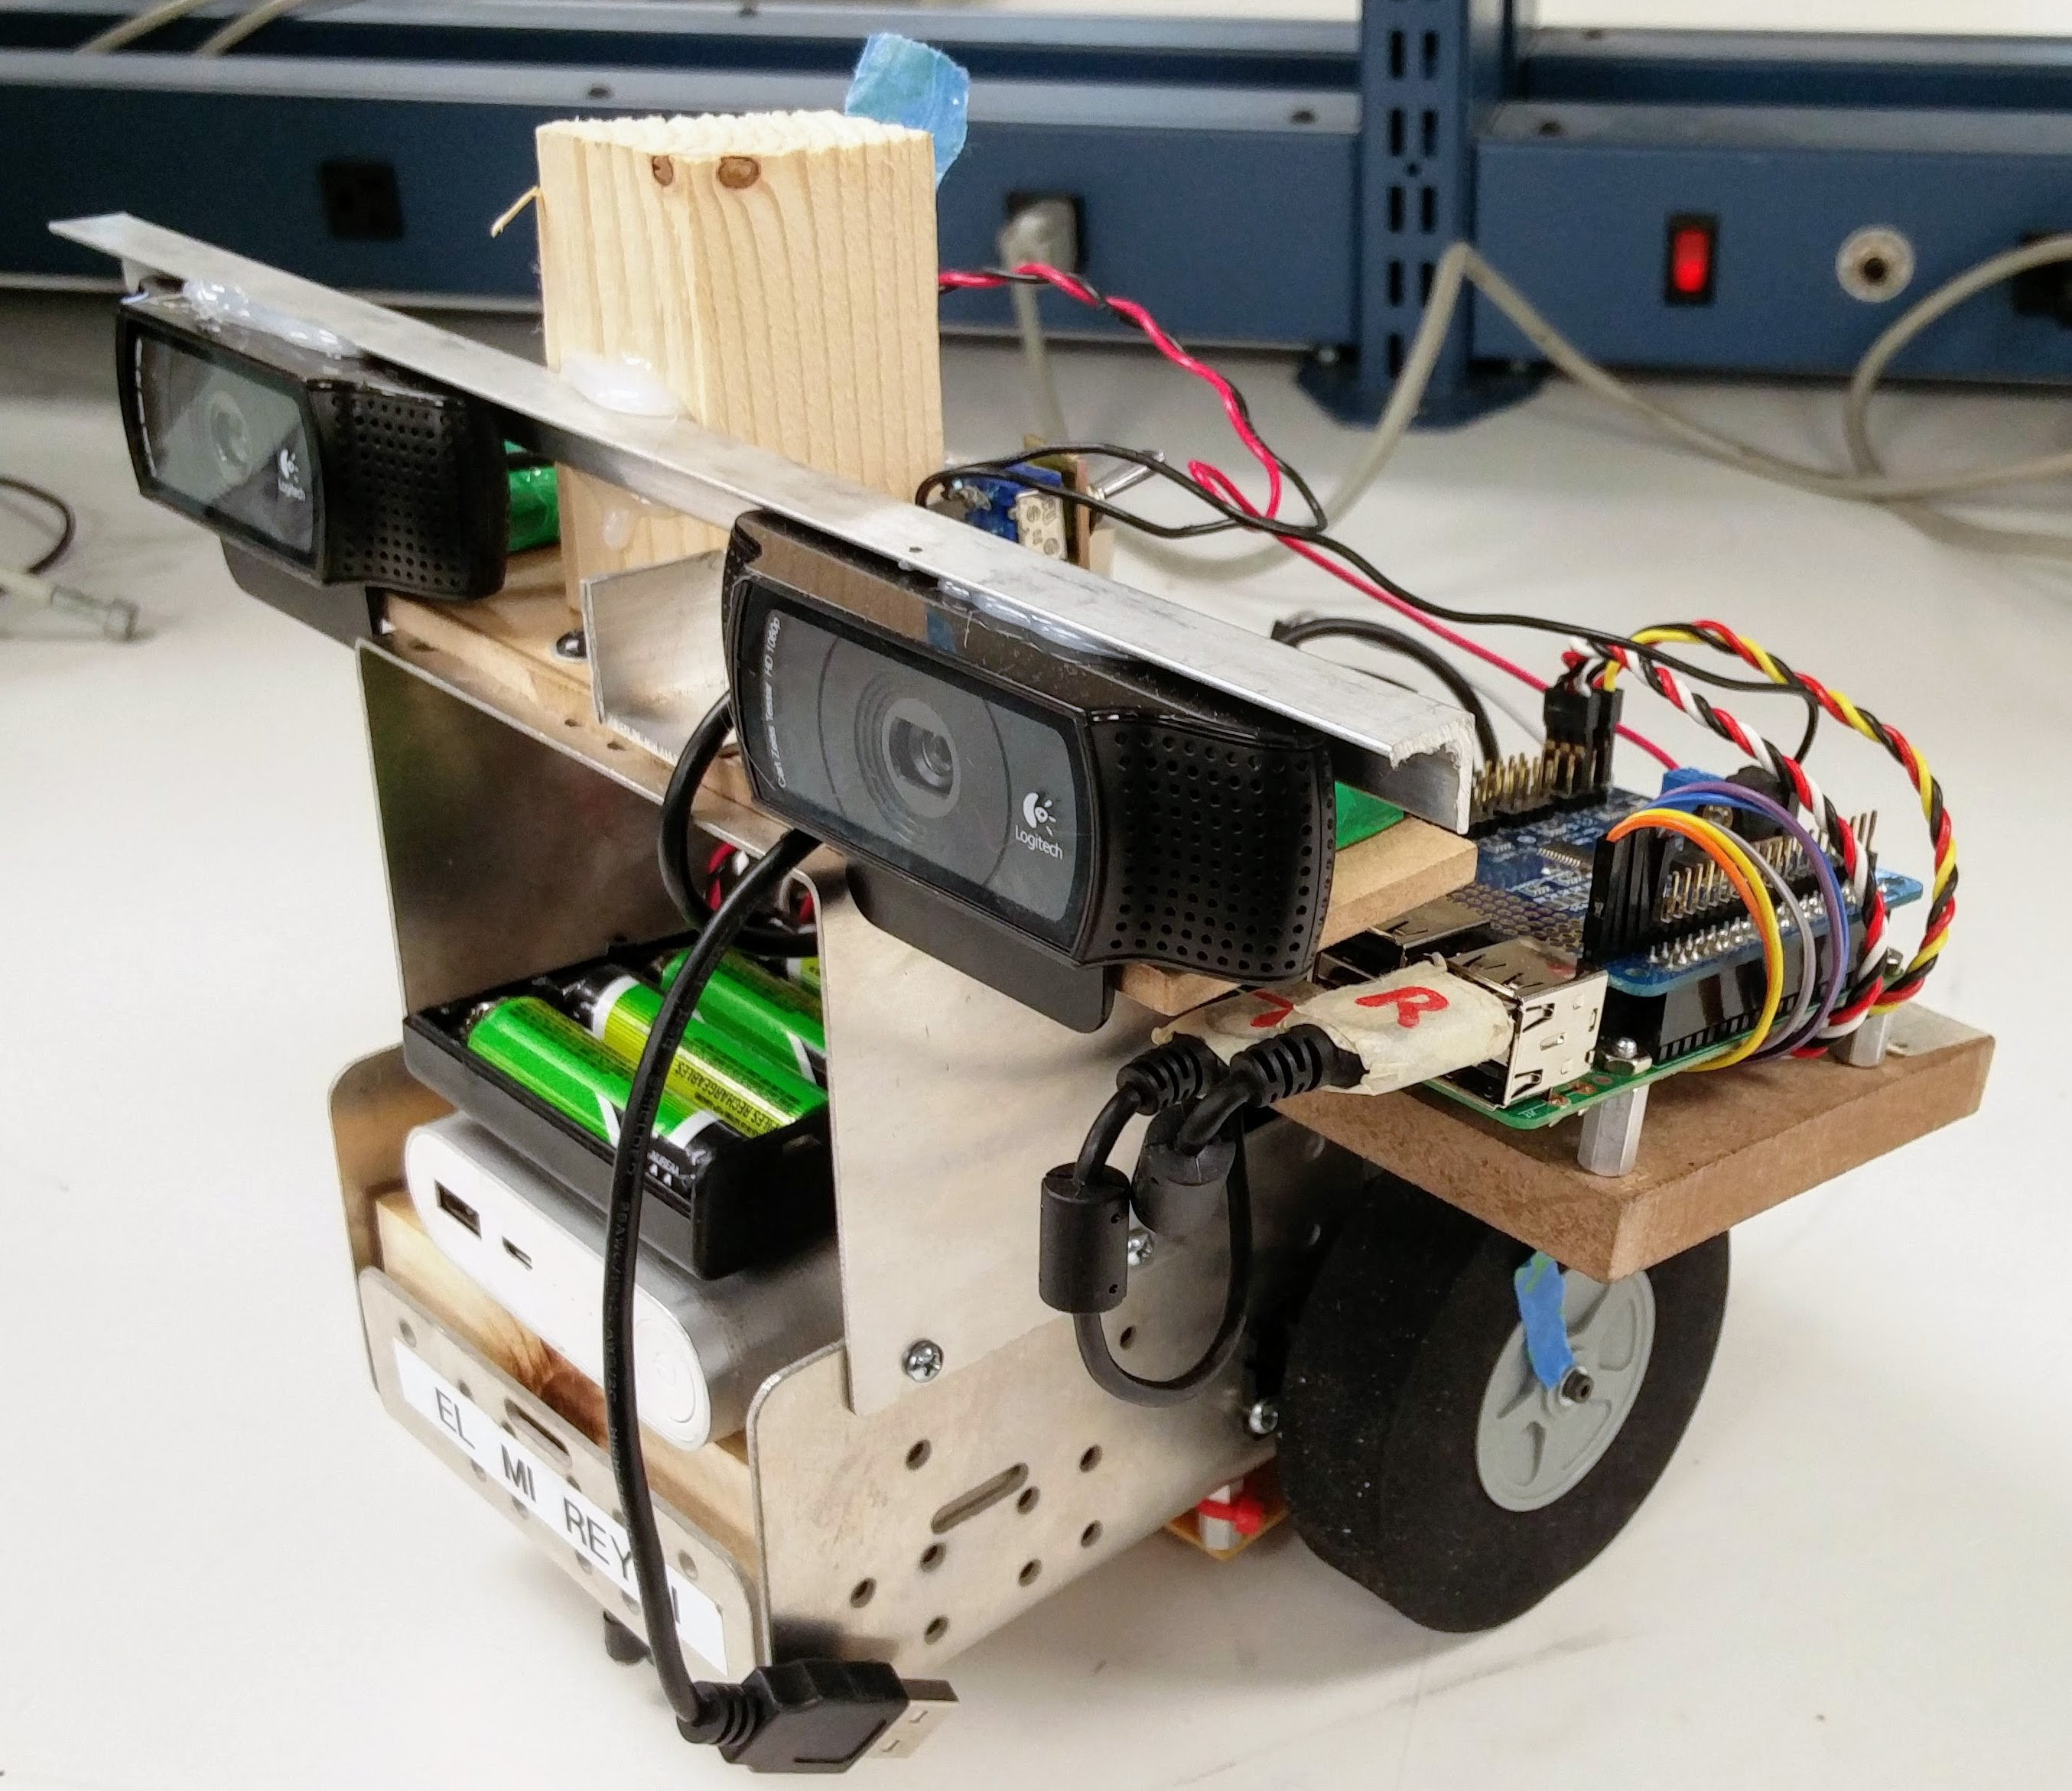
\includegraphics[width=0.5\textwidth]{Bot.jpg}
\caption{The Robot with 2 logitech webcams connected to  Raspberry Pi 3}
\end{figure*}
This solved our streaming issue. However, we now experienced a intermittent broken pipe error when starting the streaming. The issue would appear occasionally and only ever when starting the cameras. We attempted switching what USB ports we were using, what order the cameras were plugged in, and changing the camera, with no result. When we switched Pis we saw a decreases in events but not a total fix. Eventually we narrowed the issue down to a power spike when the camera was initialized causing the voltage on the USBs to sag resulting in the second camera failing. This issue can be avoided by waiting at least 20 seconds for the first camera to finish initializing before you start the second. 
\subsection{Camera Calibration and Synchronization}
Now that we had functioning streaming, we calibrated the cameras using the ROS camera\_calibration package \footnote{\href{http://wiki.ros.org/camera\_calibration}{http://wiki.ros.org/camera\_calibration}}. We then published the calibration files to ROS along with the video streams. Then we ran ORB\_SLAM2\footnote{\href{https://github.com/raulmur/ORB_SLAM2}{https://github.com/raulmur/ORB\_SLAM2}}, it successfully localized the robot, found loop closure, providing trajectory, and creating a point cloud. Next we moved on to trying to run RTAB-Map.\footnote{\href{https://introlab.github.io/rtabmap/}{https://introlab.github.io/rtabmap/}} To do this we had to run stereo\_image\_proc \footnote{\href{http://wiki.ros.org/stereo\_image\_proc}{http://wiki.ros.org/stereo\_image\_proc}} package which takes in the published stereo images and corresponding camera info and to produce rectified images, gray scale images, disparity images, and a point cloud. These are passed into RTAB which uses these and the odometry to create a map of its surroundings. Stereo\_image\_proc would not run because our left and right camera images were not synchronized. To resolve this we tried a number of modifications to our streamer. First we tried to combined the videos on the Pi and then stream them as one object, so that when they were passed into ROS they would arrive at the same time. This failed because the memory buffer allocation failed. Next we tried to use multi treading to simultaneously stream the two videos. This failed because pythons multi threading capabilities were insufficient for the heavy load. Then we progressed to the receiver. Initially we attempted to synchronize the files by re-writing the python socket receiver so that it captured the the two frames simultaneously and then passed them into ROS as one object. This failed because trying to synchronize the frame receptions was causing the stream to lag. Next, we tried to alternate the reception of the packets from both frames in the same sequentially we attempted to use the ROS message\_filter package executed script and then publish them once both were received. This failed because when receiving the frames one would block the other resulting in many incomplete frame and inconsistent image quality. Next \footnote{\href{http://wiki.ros.org/message\_filters}{http://wiki.ros.org/message\_filters}}, this did not sufficiently synchronize the images. Finally, we managed to synchronize the images by waiting until they were published into ROS, by separate receivers, and then editing the time stamp to be the same value.
\begin{figure*}[!h]
\centering \includegraphics[width=0.7\textwidth]{Pic2.jpg}\label{Occupancy Grid Created}
\caption{Occupancy Grid Created}
\end{figure*}
\subsection{SLAM and Hardware}
Once the synchronization was achieved stereo\_image\_proc worked but resulted in an image that was more distorted than the raw image. However, now that we had stereo\_image\_proc functioning we attempted to run RTAB. RTAB requires transformations from the fixed frame of the robot to the camera. For this we used an Unified Robot Description Format file. URDF is an XML format for representing a robot model. We use this file to accurately describe the robot in space, for finding the transformations between different links in the robot, and for finding the correlation between different frames of references. We also added support for the encoders. The encoder values are read using an ADC connected to the Raspberry Pi. Using motors controlled by a joystick, we were able to test the accuracy of the encoders by moving the robot in a pattern. When working with the encoders, we had an issues with the numbers increasing when the robot was not moving. To resolve this we required two reading of each color before registering a color change. After testing, we determined that the encoders were not accurate enough for our application, so we increased the number of divisions on the encoder wheels from 20 to 40. Also RTAB requires that the images be associated with a link in the robot transform. We added functionality to the synchronization node to update the associated link in the ROS message being published. 

\begin{figure*}[!h]
\centering 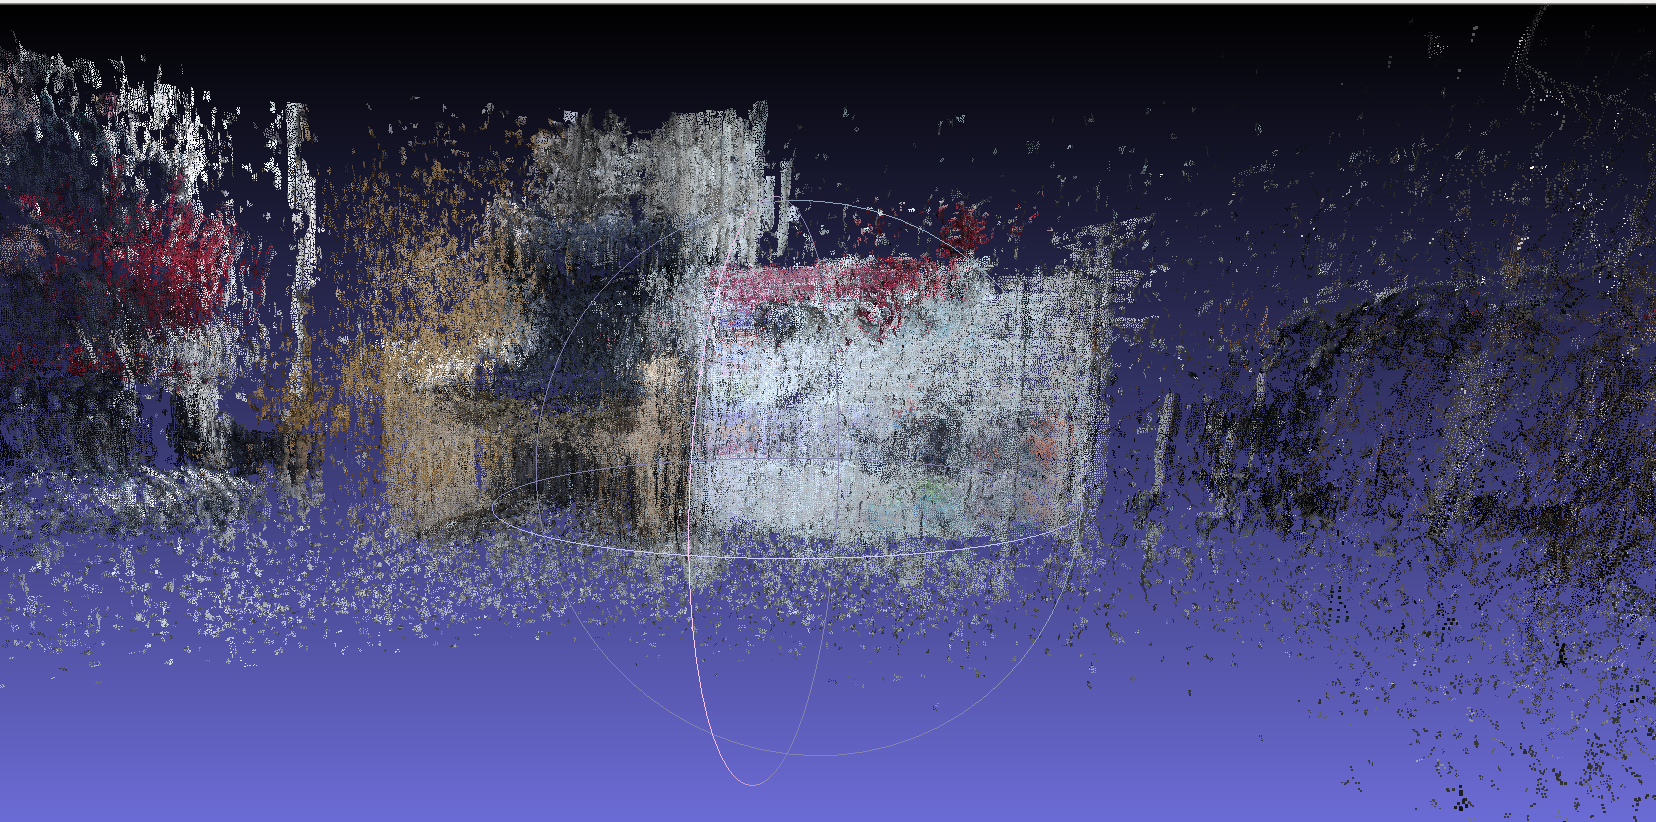
\includegraphics[width=0.7\textwidth]{PointCloud.png}\label{Point Cloud}
\caption{Point Cloud of Chair and Poster as seen by the robot}
\end{figure*}

We ran RTAB which resulted in a poor point cloud, so we re- calibrated the cameras using a larger and more precise checkerboard. During this process, one of the motors and one of the encoders failed. We replaced the motor and encoder. We tweaked the settings of the stereo\_image\_proc package to produce the best possible point cloud from the disparity in the stereo images. We were able to get a good point cloud and an average occupancy grid.(Figure 3)

\section{Experimental Results and Analysis}
\subsection{Video streaming from Raspberry pi}
	At the beginning of the project we started with ROS uvc\_camera package to stream the stereo feed to the personal computer. However , as ROS uses TCP protocol the video stream had bad performance and can be seen in the table below. The stream received was synchronized but was not good enough to run any real time algorithms as it was delayed by about 2s. One of the counter measures taken was to use gray scale images, as the SLAM algorithms do not make use of the color information in the images. The frame rate increased to 5 fps, however the delay was still the same. We then switched to UDP based streaming programs and used v4l2 based streamer. This yielded extremely good results with 800x600 images being streamed at 30FPS and a delay of less than 0.5s. However the synchronization between the frames was lost and we had to handle the synchronization at the receiver using another buffer ROS program.
\begin{figure}[H]
\centering 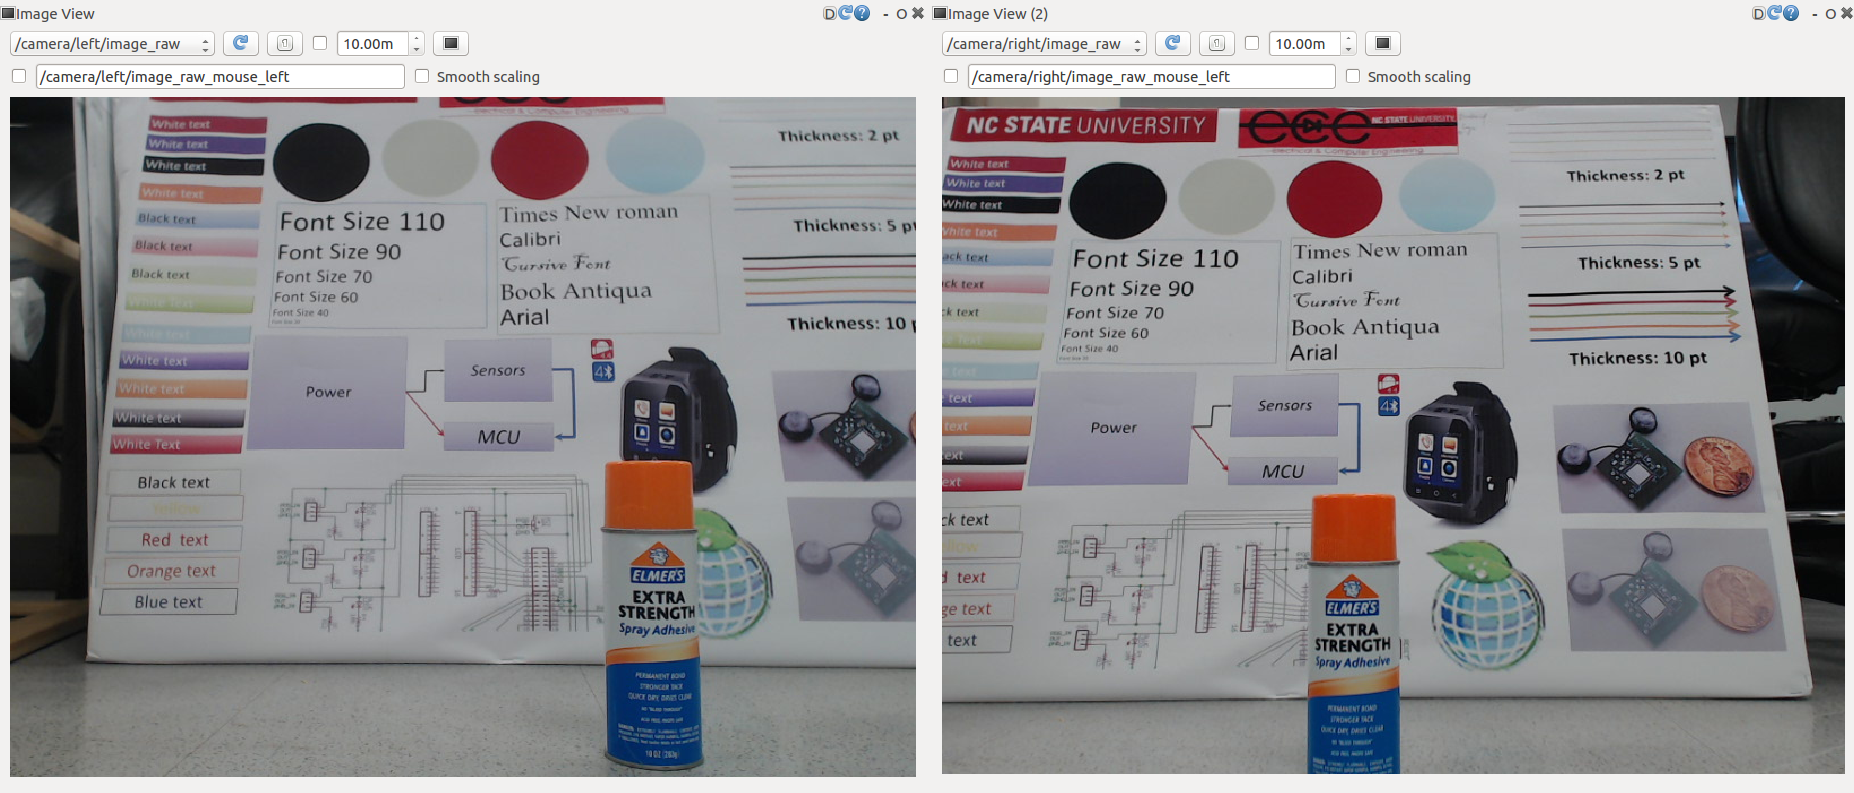
\includegraphics[width=0.7\textwidth]{stereo_view.png}\label{Stereo video feed}
\caption{Stereo video feed}
\end{figure}
\begin{table}[H]
\begin{center}
\begin{tabular}{|c|c|c|c|c|c|}
\hline
Method &FPS & Delay & Image Size & Image Consistency & Synchronization\\[1ex]
\hline
ROS uvc\_camera & 3 & 2s & 640x480 & Good & Yes\\ [1ex]
\hline 
ROS uvc\_camera Gray scale images& 5 & 2s & 640x480 & Good & Yes\\ [1ex]
\hline 
self-made UDP socket& 0 & $\infty$s & 640x480 & Bad & No\\ [1ex]
\hline 
v4l2 driver & 30 & \textless 0.5s  & 800x600 & Good & No\\ [1ex]
\hline

\end{tabular}
\caption{Stream method analysis}
\end{center}
\end{table}

\subsection{Experiments with Encoders}
When testing for the accuracy of our odometry, we noticed that the encoder values increased when the robot was stationary. In response we checked to ensure that we get multiple consistent encoder readings before registering a color change. We would still occasionally get the number increasing very rapidly. We determined that is was the result of the encoder stopping on the devision between white and black, resulting in the value being right around the threshold. To resolve this we inserted a 'dead band' which is considered neither white nor black. We also had issues with the encoders not accurately measuring turns, so we decided to create our own encoder wheel to suit our application. Hence, the 20 division encoder was replaced with a 40 devision encoder wheel. This setup increased the resolution of the encoders and allowed the odometry to consistently measure turns.     
\begin{figure}[H]
\centering 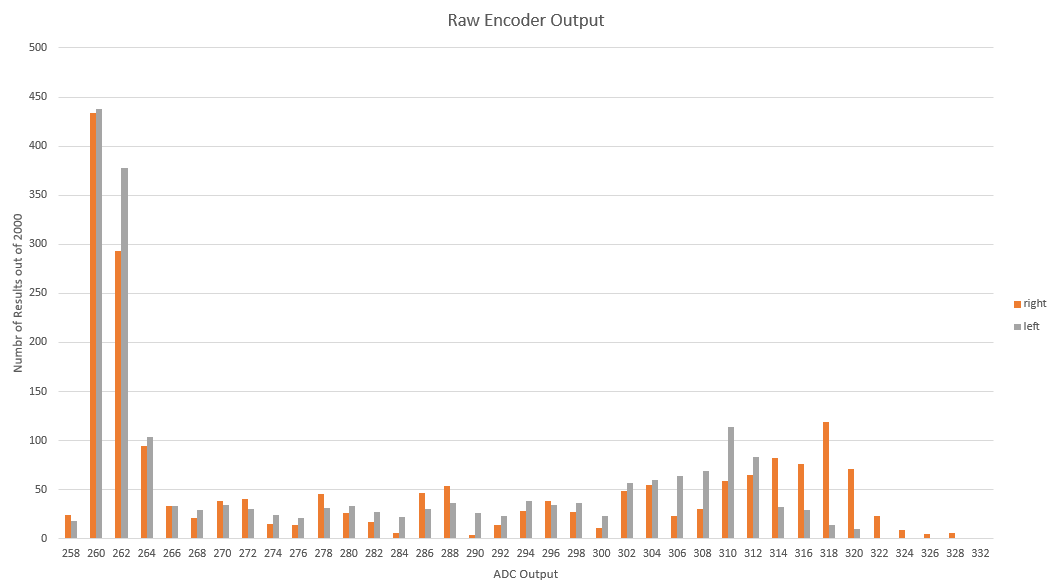
\includegraphics[width=0.6\textwidth]{EncoderValues.png}\label{Encoder values}
\caption{Histogram Encoder values}
\end{figure}


\subsection{Camera Calibration Results}
	Calibration of images is one of the most important part of any computer vision applications. This process yields a list of values which are used to correct the image of distortions due to the inherent defects in the sensor and lenses. One of the common ways of calibration is to use a checkerboard pattern and estimate the parameters based on the corners in the checkerboard. The number and size of square are input to the calibration function. We have used the ROS calibration program to do this. We first tried the calibration using a 9x7 checkerboard with 25mm squares. The results were not as good and can be seen in Figure 6. The calibration was repeated with a big checkerboard with 9x6 113mm squares. The result is a good rectified image as can be seen in Figure 7. The result is not perfect and requires fixing both web cameras onto a single platform and ensuring there is no motion relative to each other. The current calibration was done using 39 image pairs. Higher number of images yield better results but take significantly longer time.
    
\begin{figure}[H]
\centering \includegraphics[width=0.7\textwidth]{Pic1.png}\label{Chekerboard}
\caption{Calibration in Progress, detected Checkerboard corners are highlighted by program}
\end{figure}

\begin{figure}[H]
\centering 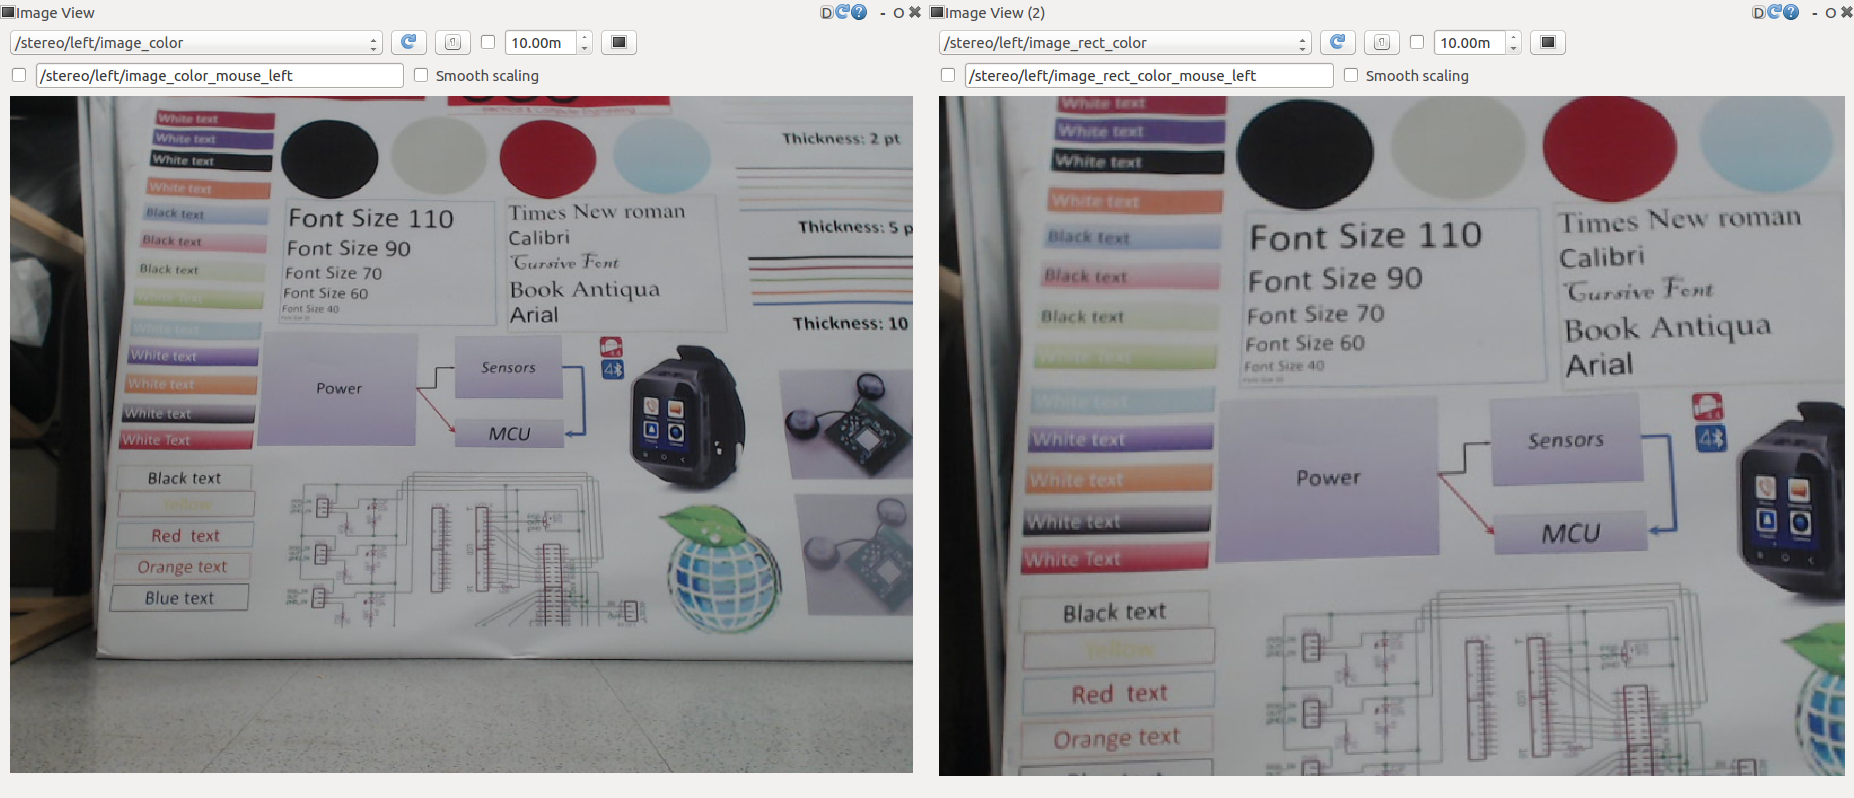
\includegraphics[width=1\textwidth]{BadCalibration.png}\label{Result Bad Calibration}
\caption{Poor Calibration , right image is the rectified image of the left image}
\end{figure}

\begin{figure}[H]
\centering 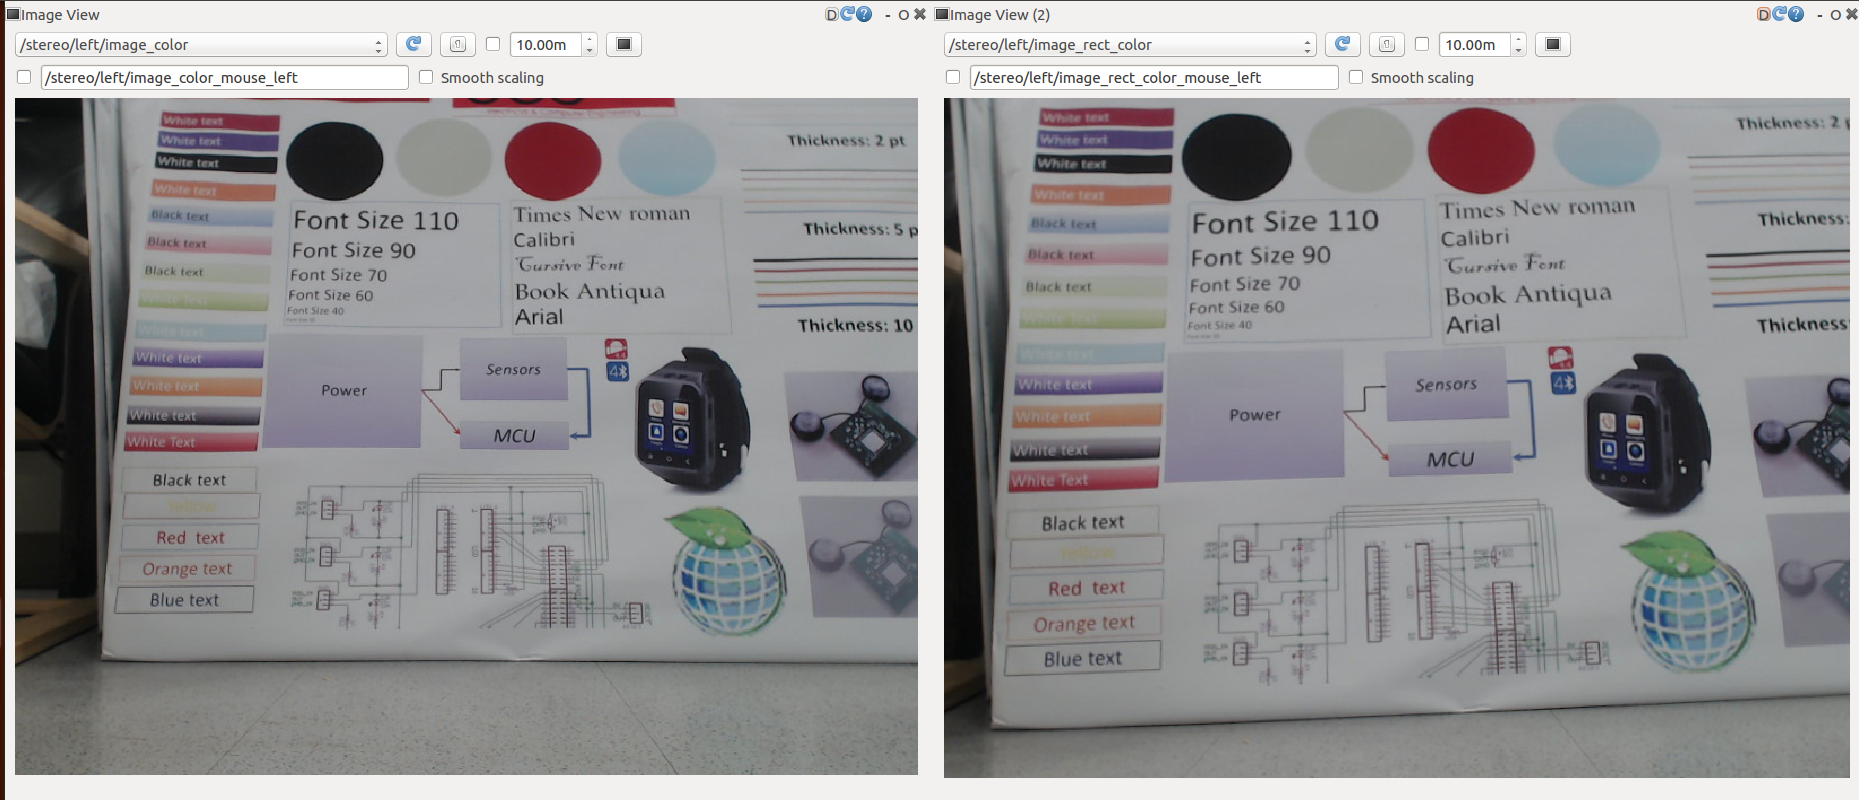
\includegraphics[width=1\textwidth]{GoodCalibration.png}\label{Result Good Calibration}
\caption{Good Calibration , right image is the rectified image of the left image}
\end{figure}

\subsection{Stereo\_Image\_Proc Calibration Results}
Stereo\_Image\_Proc is used to produce a disparity image by comparing the right and left camera stream. By adjusting the perimeters it uses you can tailor the setting to fit your objective. These allow for you to filter out noise in the environment, control the sensitivity to texture, and control the intended focus length of the cameras. In figure 9 you can see the improvement after fine tuning of these settings.    
\begin{figure}[H]
\hfill
\subfigure[Initial Stereo\_Image\_Proc Point Cloud]{\includegraphics[width=7cm]{Pic.png}}
\hfill
\subfigure[Final Stereo\_Image\_Proc Point Cloud]{\includegraphics[width=7cm]{Pic6-edited-2.jpg}}
\hfill
\caption{Initial Stereo\_Image\_Proc Calibration}
\end{figure}






\subsection{ORB SLAM Results}
	With the Stereo feed available we tested ORBSLAM2. ORBSLAM2 is well known for robustness,good localization and real-time performance. However the point cloud generated was not good and the environment cannot be known. With our setup we were able to get a good loop  closure and odometry and can be used to supplement wheel odometry.The results can be seen in Figure  11.\footnote{\href{https://www.youtube.com/watch?v=LTfOwyYde9E}{https://www.youtube.com/watch?v=LTfOwyYde9E}}
\begin{figure}[H]
\centering 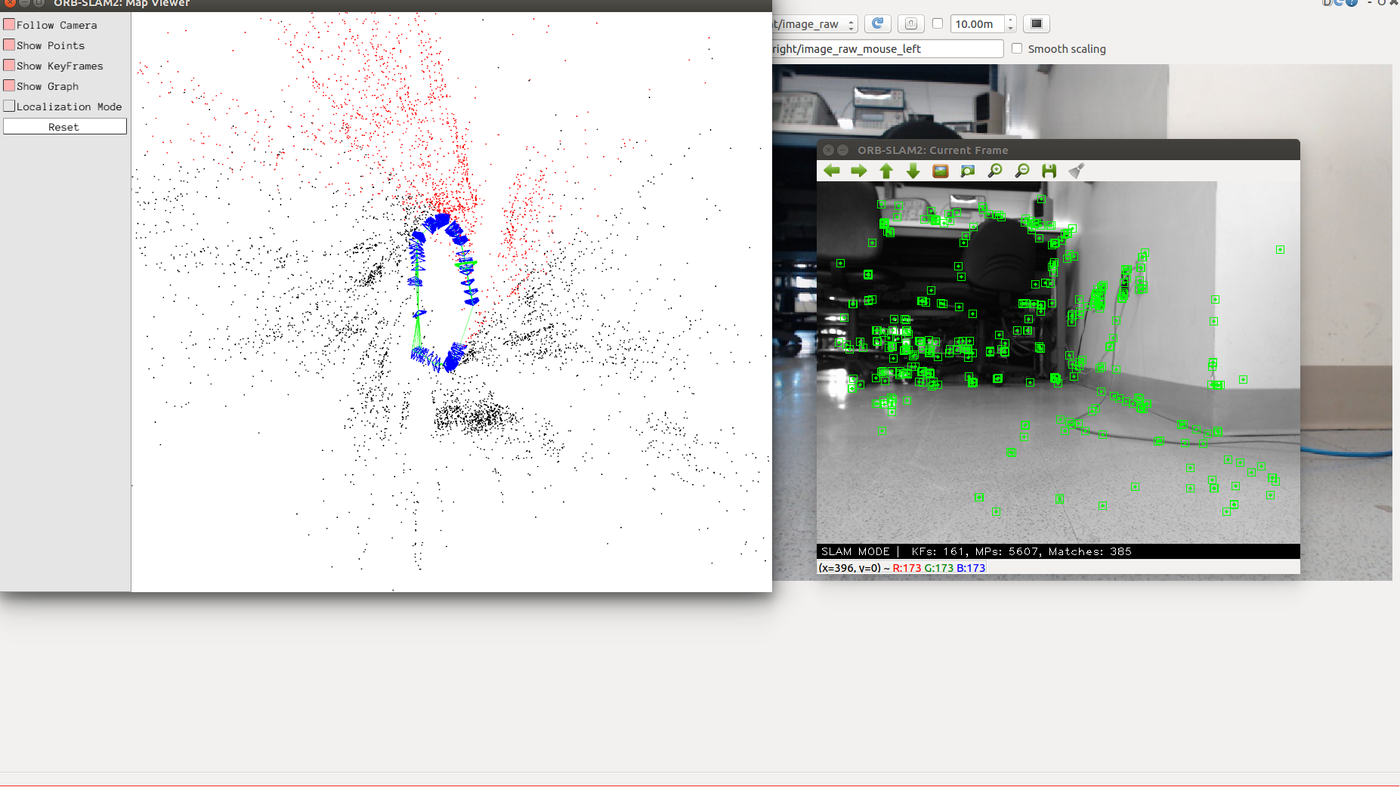
\includegraphics[width=1\textwidth]{ORBSLAM.png}\label{ORBSLAM2}
\caption{loop closure with ORBSLAM}
\end{figure}

\subsection{RTAB Map Results}
	While ORBSLAM can provide good and robust Odometry in realtime, RTAB can create a good 3D point cloud of the environment and a occupancy grid. It does this by using rectified images from stereo\_image\_proc and odometry. It projects the point onto a plane to create a occupancy grid. The settings for the height of obstacle can be changed and only objects of certain height can be treated ass obstacles. The occupancy grid created can be used for navigation.
\begin{figure}[H]
\centering 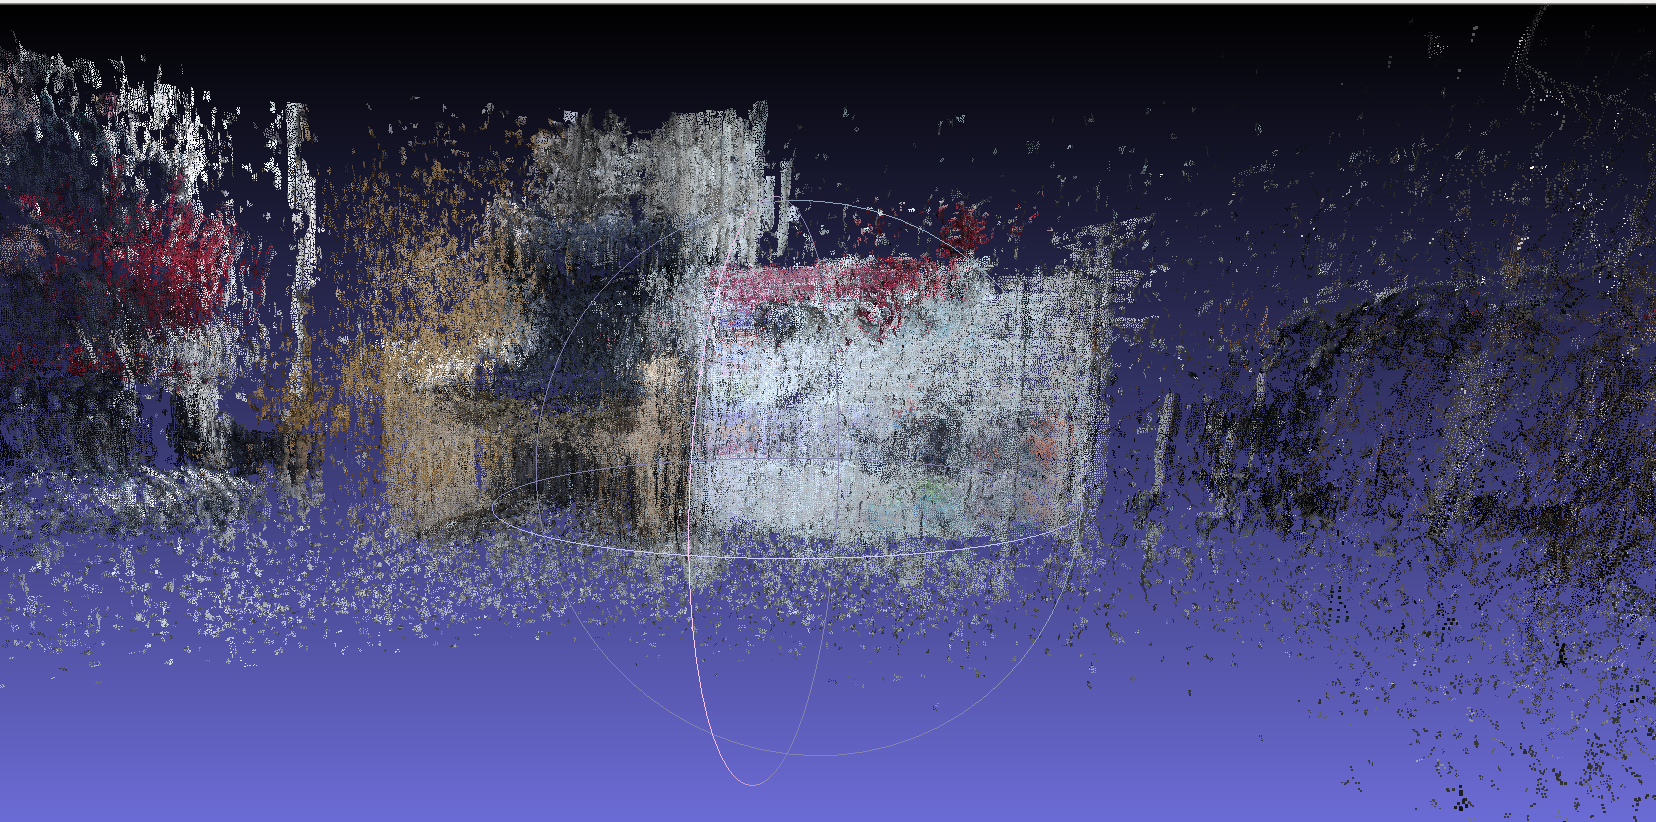
\includegraphics[width=1\textwidth]{PointCloud.png}\label{PointCloud of RTAB}
\caption{Point Cloud of RTAB shows a chair on the side and a poster beside it rendered in 3D.}
\end{figure}
\begin{figure}[H]
\centering 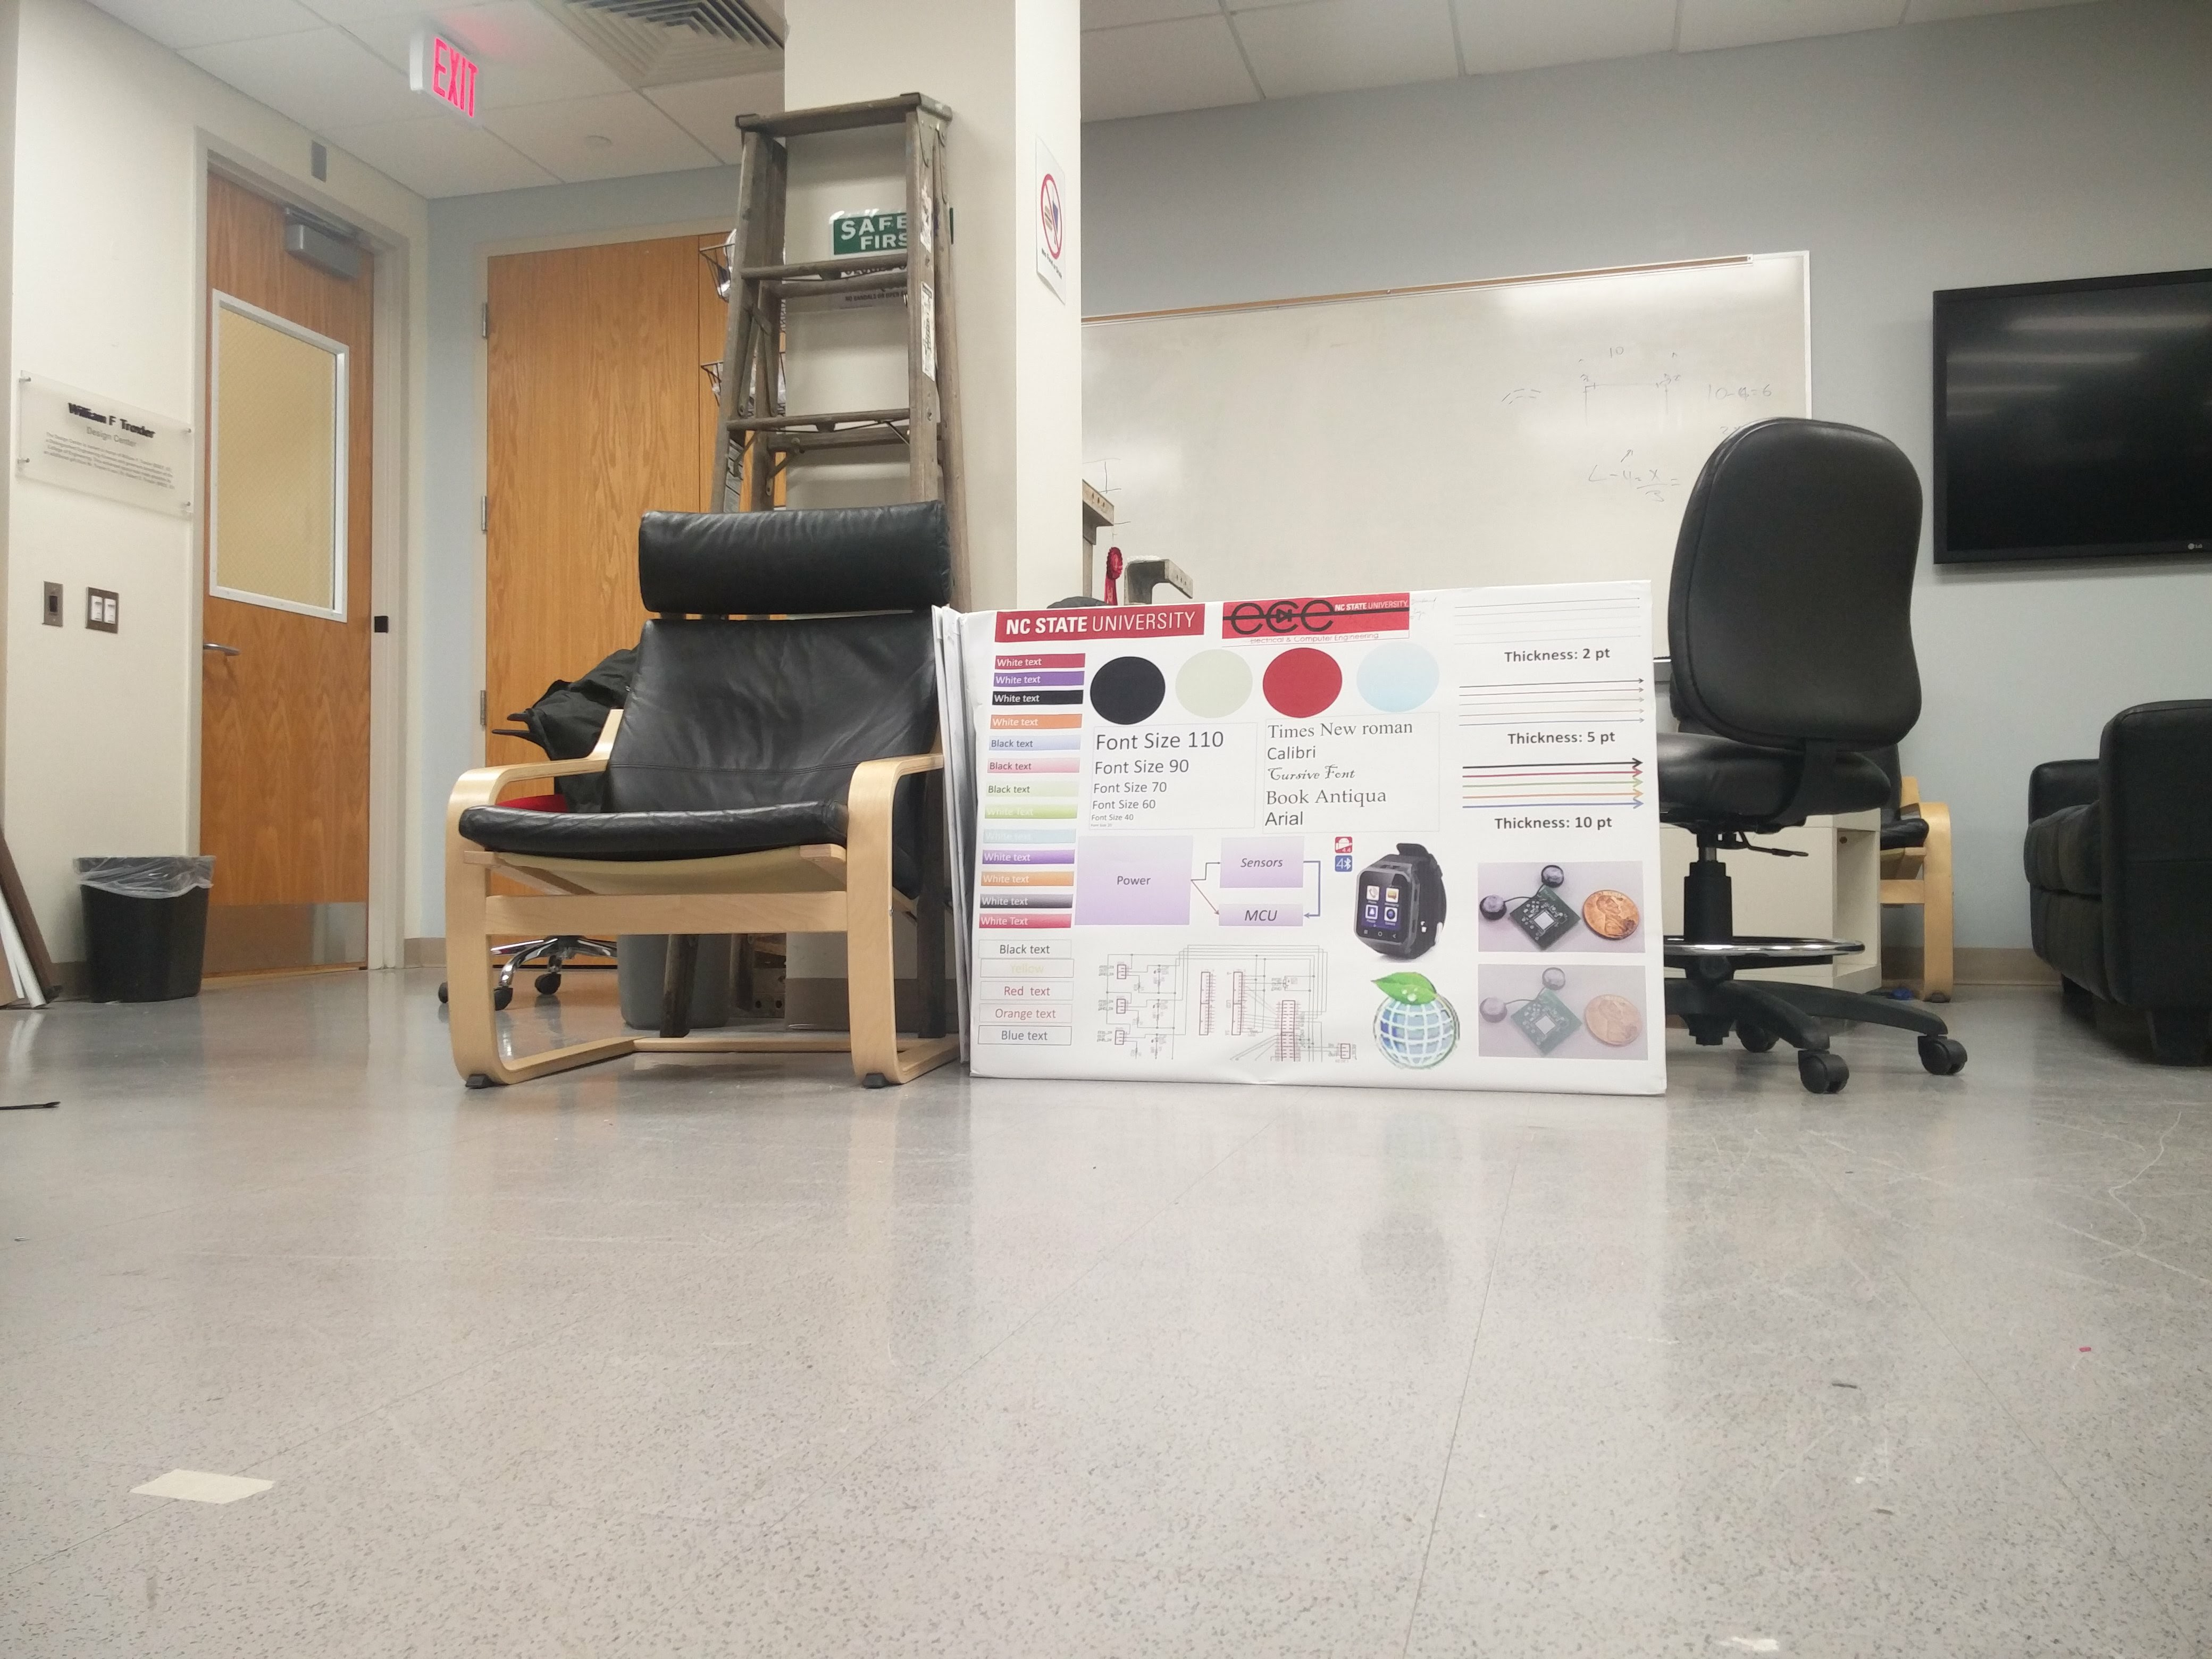
\includegraphics[width=0.7\textwidth]{chair.jpg}\label{Point Cloud Image}
\caption{The scene reconstructed by RTAB.}
\end{figure}
\begin{figure}[H]
\centering \includegraphics[width=1\textwidth]{Pic8.jpg}\label{Occupancy Grid}
\caption{Occupancy Grid created using RTAB. The black color indicates obstacles and rest is traversable space}
\end{figure}


\pagebreak
\section{Conclusion}
The problem statement was to implement a low cost Indoor SLAM for scanning an indoor area using a camera(s) and create a 3D reconstruction of its environment and also to create an occupancy grid or a traversable map. We were able to transform a two wheeled robot skeleton with motors and wheels into a robotic platform to stream stereo images to a remote computer and capable of controlling the motors on receiving commands form the remote computer. We were able to recreate the environment around the robot as a three dimensional point cloud. To achieve this level of performance, we had to create our own stereo camera rig using two monocular USB cameras. We implemented a python socket program to stream the video feed. We have implemented two SLAM techniques and compared their results for our robotic setup. 
%\pagebreak
\section{Appendices}
\subsection{GitHub repository}

All source code and instructions to recreate the project can be accessed from the GitHub repository Indoor\_SLAM \href{https://github.com/surajshanbhag/Indoor\_SLAM.git}{https://github.com/surajshanbhag/Indoor\_SLAM.git}
\subsection{Supplementary Images}
\begin{figure}[H]
\hfill
\subfigure[Old encoder]{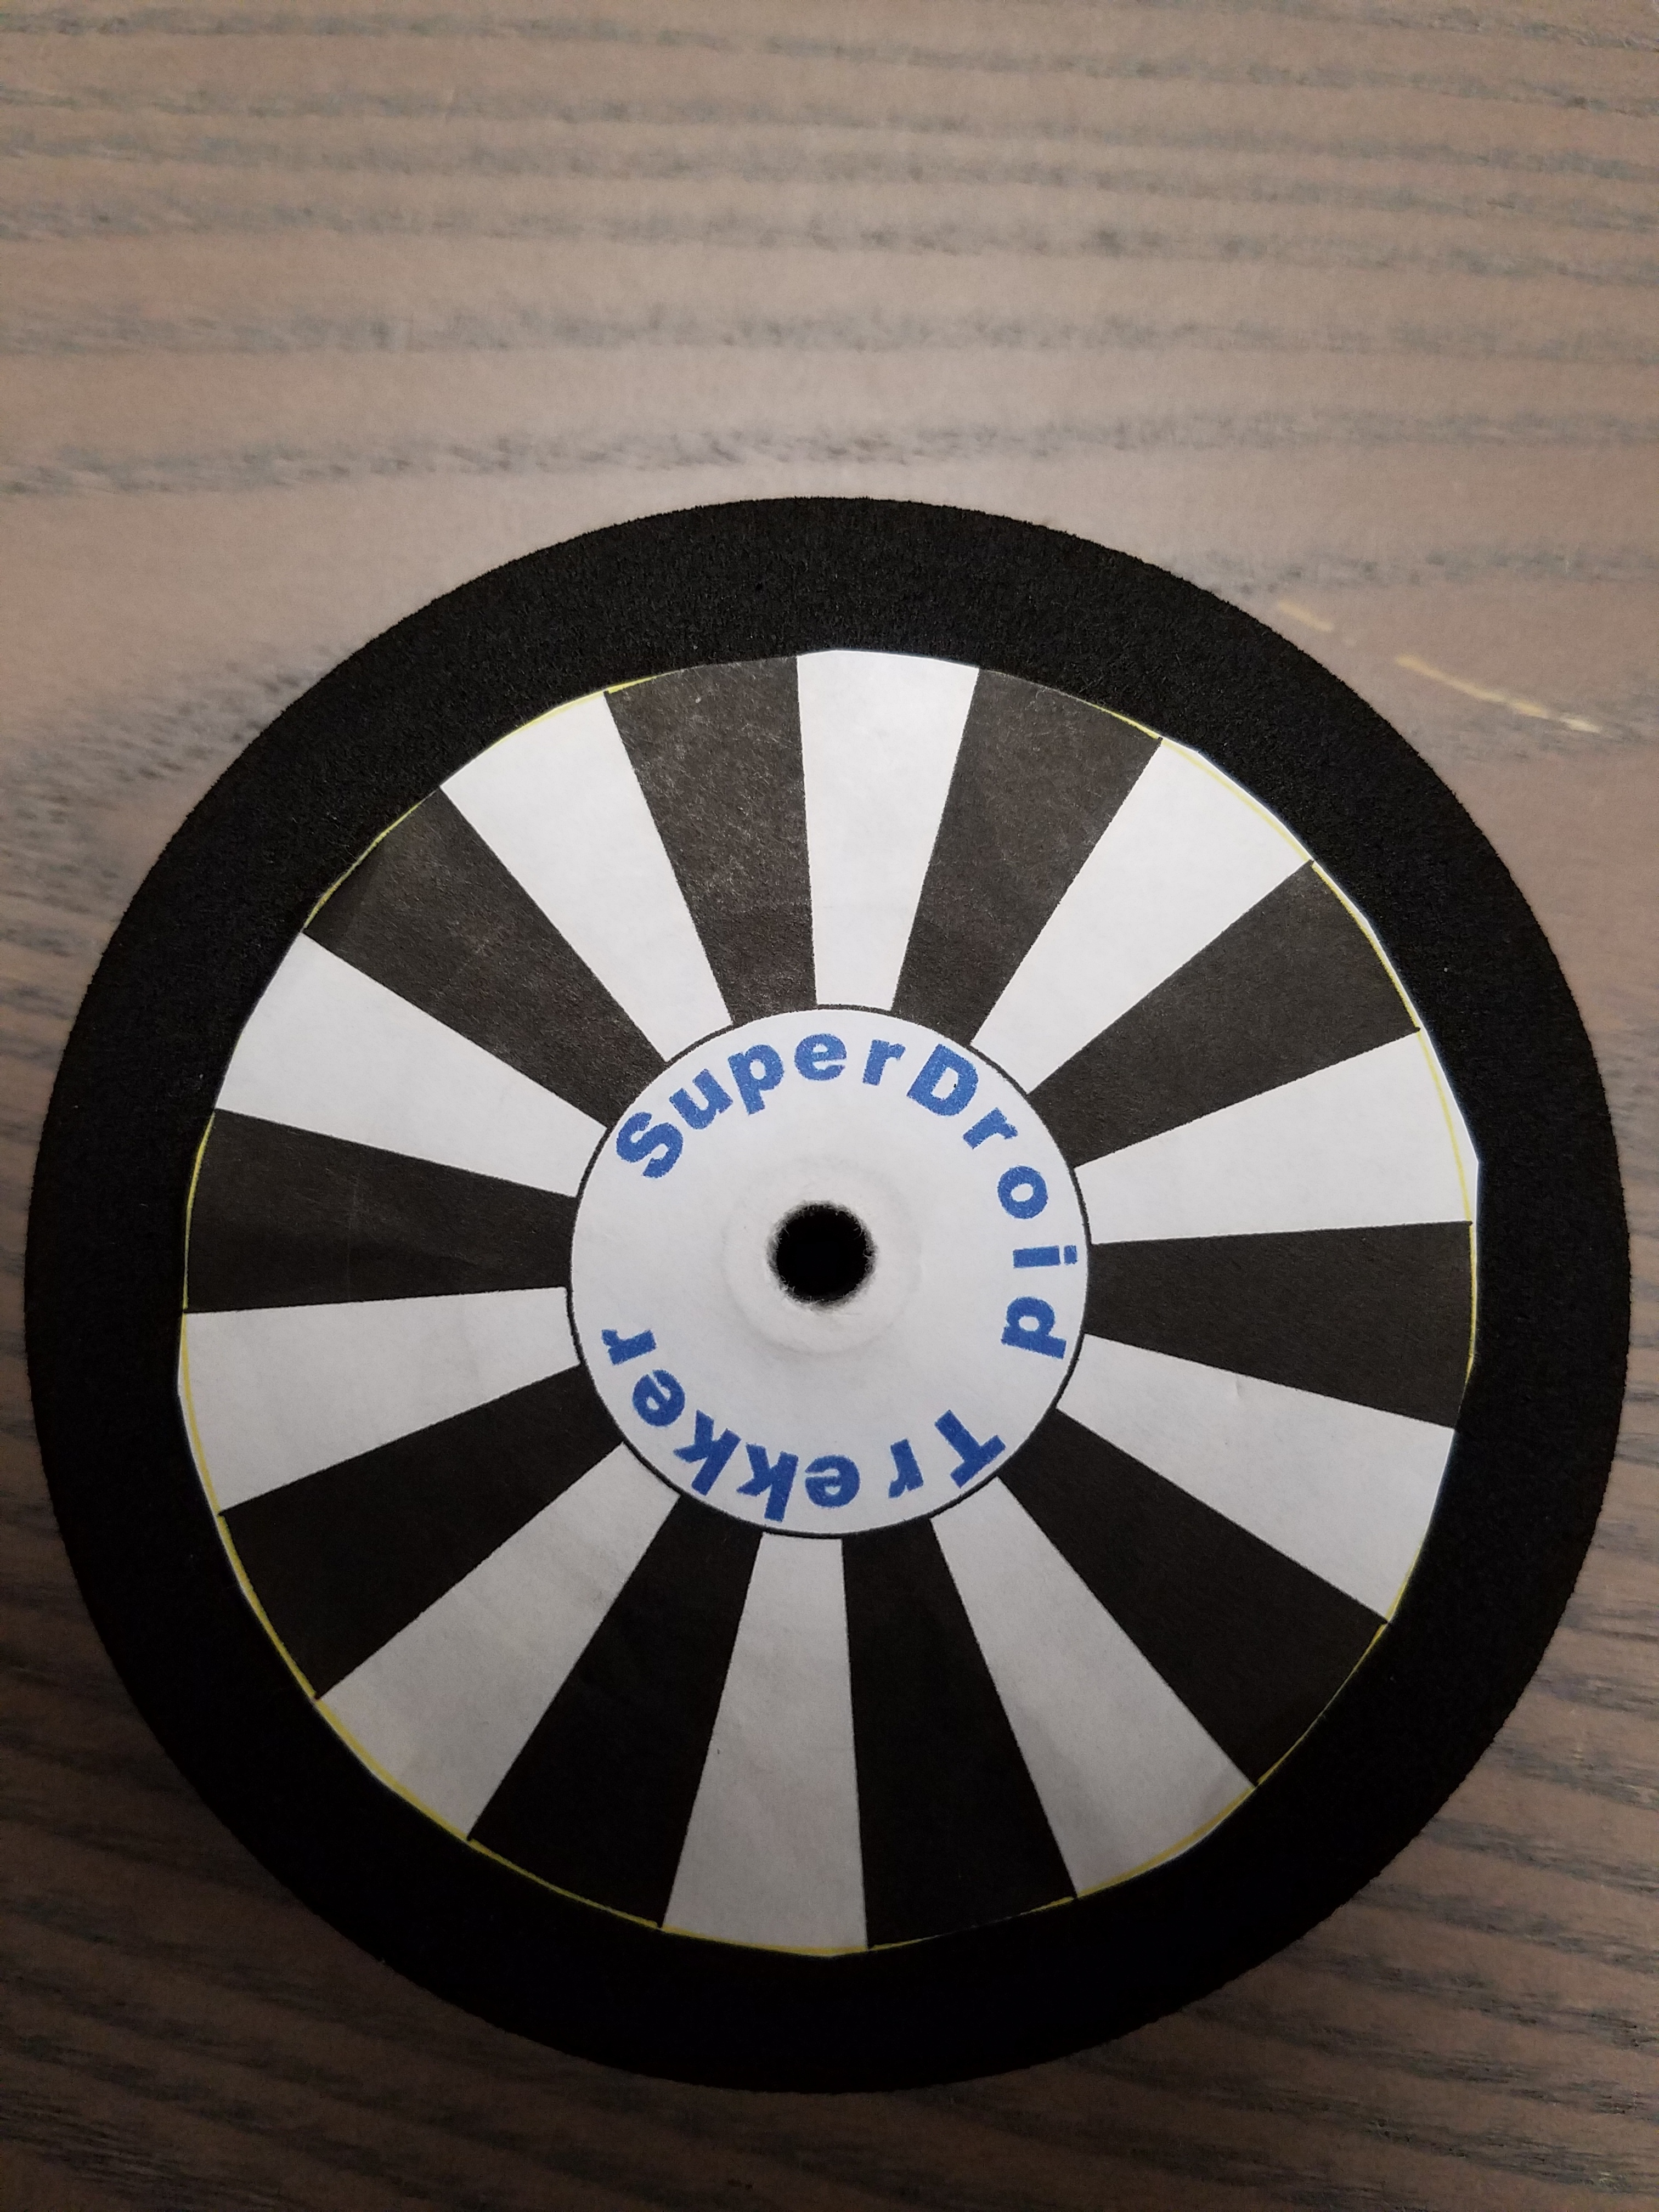
\includegraphics[width=5cm]{oldencoder.jpg}}
\hfill
\subfigure[New encoder]{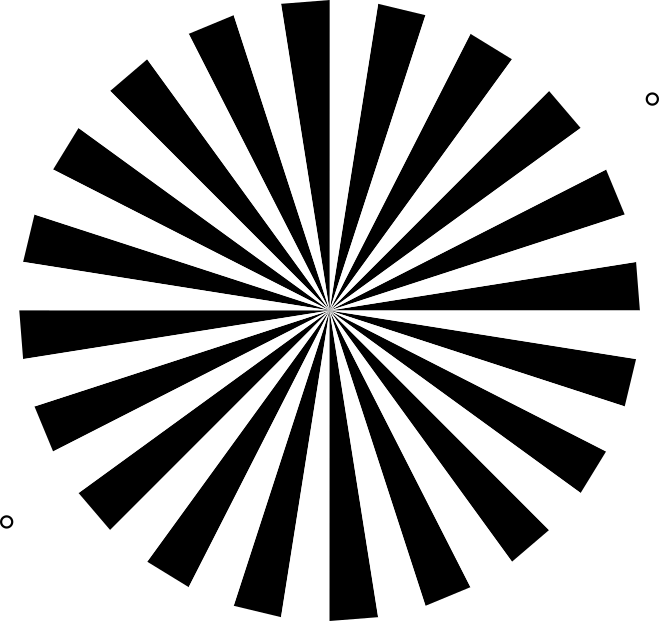
\includegraphics[width=5cm]{encoder.png}}
\hfill
\caption{Encoder stripes}
\end{figure}
\begin{figure}[H]
\centering 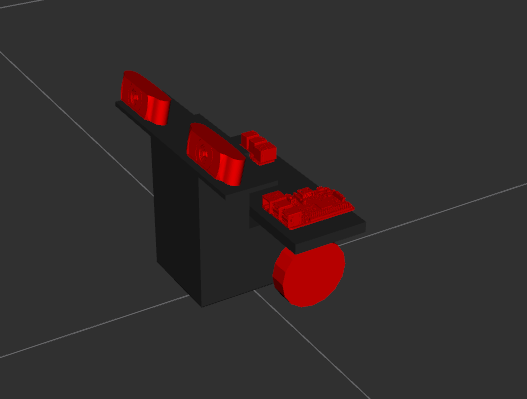
\includegraphics[width=0.5\textwidth]{urdf.png}\label{URDF Model}
\caption{URDF Model created for the project. Provides frame of references and transformation between wheels, cameras and the base of the robot.}
\end{figure}
\bibliographystyle{unsrt}
\end{document}
